\chapter{Analiza wyników, możliwe drogi dalszego rozwoju}~\label{results_analysis_chapter}
% \section{Zasady redakcji}
% W pracy należy dbać o poprawność redakcyjną zgodnie z zaleceniami:
% \begin{itemize}
% \item nie zostawiać znaku spacji przed znakami interpunkcji (zamiast ,,powiedziano , że ...'' powinno być ,,powiedziano, że ...''),
% \item kropki po skrótach, które nie są jednocześnie kropkami kończącymi zdanie sklejać z kolejnym wyrazem znakiem tyldy, np.~jak tutaj (\verb?np.~jak tutaj?) lub wstawiać za nimi ukośnik, np.\ jak tutaj (\verb?np.\ jak tutaj?),
% \item nie zapominać o formatowaniu wyliczenia (należy zaczynać małymi literami lub dużymi oraz kończyć przecinkami, średnikami i kropkami -- w zależności od kontekstu danego wyliczenia),
% \item nie zostawiać samotnych literek na końcach linii  (można je ,,skleić'' z wyrazem następnym stosując znaczek tyldy, jak \verb+w~przykładzie+),
% \item nie zostawiać pojedynczych wierszy na końcu lub początku strony (należy kontrolować ,,sieroty'' i ,,wdowy''),
% \item nie zostawiać odstępu pomiędzy tekstem a nawiasami czy znakami cudzysłowów (znaki te powinny przylegać do tekstu, który obejmują ,,jak w tym przykładzie''),
% \item wyrazy obcojęzyczne powinny być pisane czcionką pochyłą (preferowane \verb|\emph{}|) wraz ze skrótem oznaczającym język, w szczególności ma to zastosowanie przy rozwijaniu skrótów, np.~OGC (ang.~\emph{Open Geospatial Consortium}) (w kodzie latexowym wygląda to tak: \verb|np.~OGC (ang.~\emph{Open Geospatial Consortium})|),
% \item każdy zastosowany skrót powinien zostać rozwinięty podczas pierwszego użycia, później może już występować bez rozwinięcia (skrót i jego rozwinięcie powinny trafić również do wykazu \emph{Skróty}, jeśli taki wykaz jest dołączany do dokumentu),
% \item nie wolno zostawiać zbyt dużo białej przestrzeni bez żadnego uzasadnienia. 
% \end{itemize}

% Odnosząc się do ostatniej zasady, to przekłada się ona na gospodarowanie białą przestrzenią. Poniżej przedstawiono przykład złego użycia listy wyliczeniowej. Jeśli bowiem elementy na liście są reprezentowane przez krótki tekst, to wtedy powstaje biała plama. Widać to szczególnie przy długich listach.
% \begin{quotation}
% 	\noindent Moje ulubione kolory to:
% 	\begin{itemize}
% 	\item biały,
% 	\item niebieski,
% 	\item czerwony.
% 	\end{itemize}
% \end{quotation}

% Dużo lepiej w takim przypadku albo po prostu wyliczyć wartości po przecinkach:
% \begin{quotation}
% 	\noindent Moje ulubione kolory to: biały, niebieski, czerwony.
% \end{quotation}
% albo wypisać listę w kilku kolumnach:
% \begin{quotation}
% 	\noindent Moje ulubione kolory to:
% \begin{multicols}{3}
% 	\begin{itemize}
% 	\item biały,
% 	\item niebieski,
% 	\item czerwony.
% 	\end{itemize}
% \end{multicols}
% \end{quotation}



% \section{Rysunki}
% W niniejszym szablonie numeracja rysunków odbywa się automatycznie według następujących reguł: rysunki powinny mieć numerację ciągłą w obrębie danego rozdziału, sam zaś numer powinien składać się z dwóch liczb rozdzielonych kropką. Pierwsza liczbą ma być numer rozdziału, drugą -- kolejny numer rysunku w rozdziale. Przykładowo: pierwszy rysunek w rozdziale 1 powinien mieć numer 1.1, drugi -- numer 1.2 itd., pierwszy rysunek w rozdziale 2 powinien mieć numer 2.1, drugi -- numer 1.2 itd. Wszystko to załatwia szablon. 

% Rysunki powinny być wyśrodkowane na stronie wraz z podpisem umieszczonym na dole. Podpisy nie powinny kończyć się kropką. Czcionka podpisu powinna być mniejsza od czcionki tekstu wiodącego o 1 lub 2 pkt (w szablonie jest to czcionka rozmiaru \texttt{small}). Ponadto należy zachowywać odpowiedni odstęp między rysunkiem, podpisem rysunku a tekstem rozdziału. Przykłady, jak to zrobić, zamieszczono w szablonie.

% W~przypadku korzystania z szablon odstępy te regulowane są automatycznie. Podpis i grafika muszą stanowić jeden obiekt. Chodzi o to, że w edytorach tekstu typu Office podpis nie scala się z grafiką i czasem trafia na następną stronę, osieracając grafikę. Korzystającym z niniejszego szablonu i otoczenia \verb?\figure? takie osierocenie nigdy się nie zdarzy.  

% Do każdego rysunku musi istnieć odwołanie w tekście (inaczej mówiąc: niedopuszczalne jest wstawienie do pracy rysunku bez opisu). Odwołania do rysunków powinny mieć postać: ,,Na rysunku~3.3 przedstawiono...'' lub ,,... co ujęto na odpowiednim schemacie (rys.~1.7)''. 

% Jeśli odwołanie stanowi część zdania, to wtedy wyraz ,,rysunek'' powinien pojawić się w całości. Jeśli zaś odwołanie jest ujęte w nawias (jak w przykładzie), wtedy należy zastosować skrót ,,rys.''. Jeśli do stworzenia obrazka wykorzystano jakieś źródła, to powinny one być zacytowane w podpisie tegoż rysunku. 

% Należy pamiętać o tym, że ,,rysunki'' to twory nieżywotne. W związku z tym nie mogą ''pokazywać''. Dlatego ,,rysunek~1.1 pokazuje ...'' jest stylistycznie niepoprawne. Zamiast tego zwrotu trzeba użyć ,, na rysunku~1.1 pokazano ...''.

% Rysunki można wstawiać do pracy używając polecenia \verb|\includegraphics|. Zalecane jest, aby pliki z grafikami były umieszczane w katalogach 
% odpowiadających numerom rozdziałów czy literom dodatków: \verb|rys01|, \verb|rysA| itd. Sposób wstawiania rysunków do pracy zademonstrowano na przykładze rysunków~\ref{fig:kanji-giri} i \ref{fig:alfabeta}.

% \begin{lstlisting}[label=list:includegraphics,caption=Kod źródłowy przykładów wstawiania rysunków do pracy,basicstyle=\footnotesize\ttfamily]
% \begin{figure}[ht]
%  \centering
%   
\includegraphics[width=0.3\linewidth]{rys05/kanji-giri}
%  \caption{Dwa znaki kanji - giri}
%  \label{fig:kanji-giri}
% \end{figure}

% \begin{figure}[htb]
%  \centering
%   \begin{tabular}{@{}ll@{}}
%   a) & b) \\
%   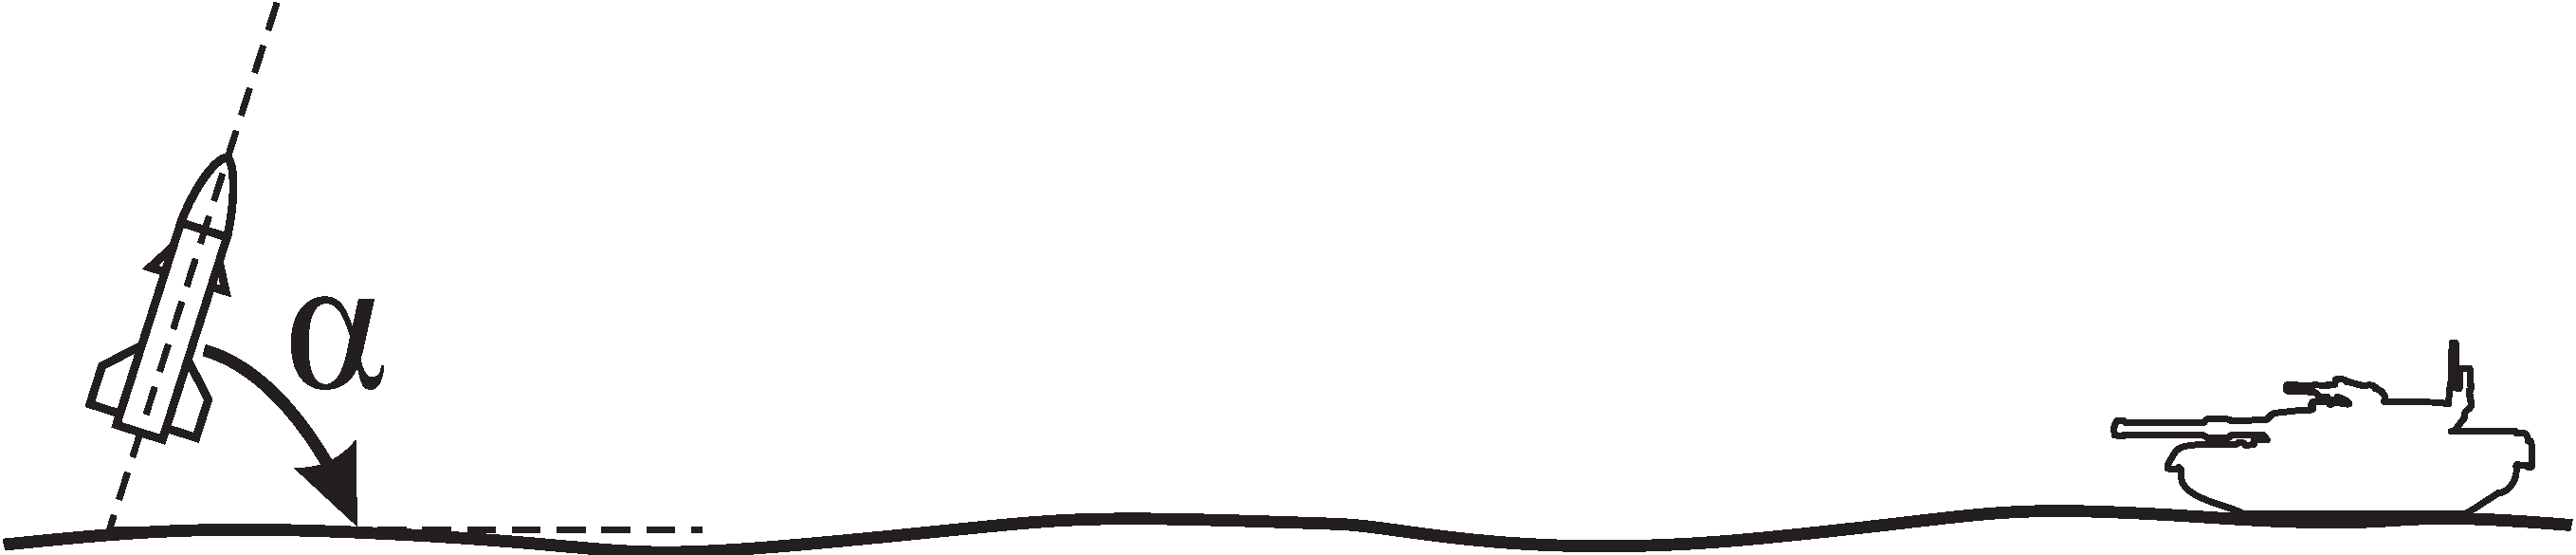
\includegraphics[width=0.475\textwidth]{rys05/alfa1} & 
%   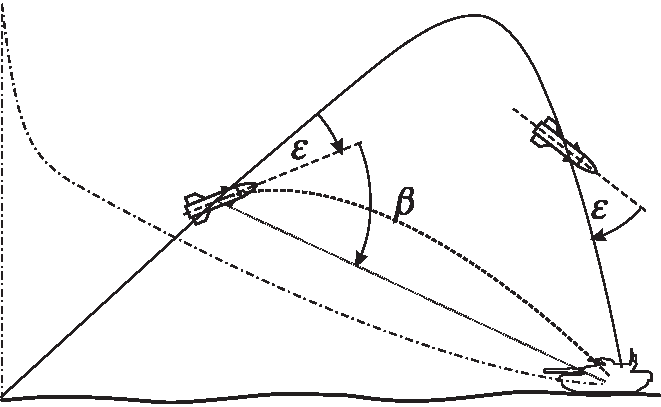
\includegraphics[width=0.475\textwidth]{rys05/beta1}
% 	% jeśli obraki są różnej wysokości, można je wyrównać do góry stosując vtop jak niżej
% 	% \vtop{\vskip-2ex\hbox{{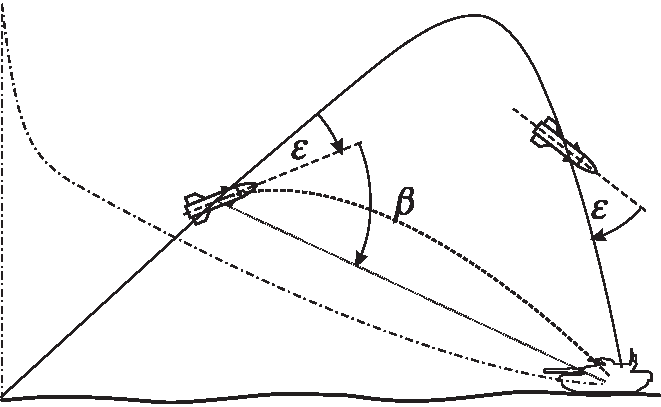
\includegraphics[width=0.475\textwidth]{rys05/beta1}}}} &
% 	% \vtop{\vskip-2ex\hbox{{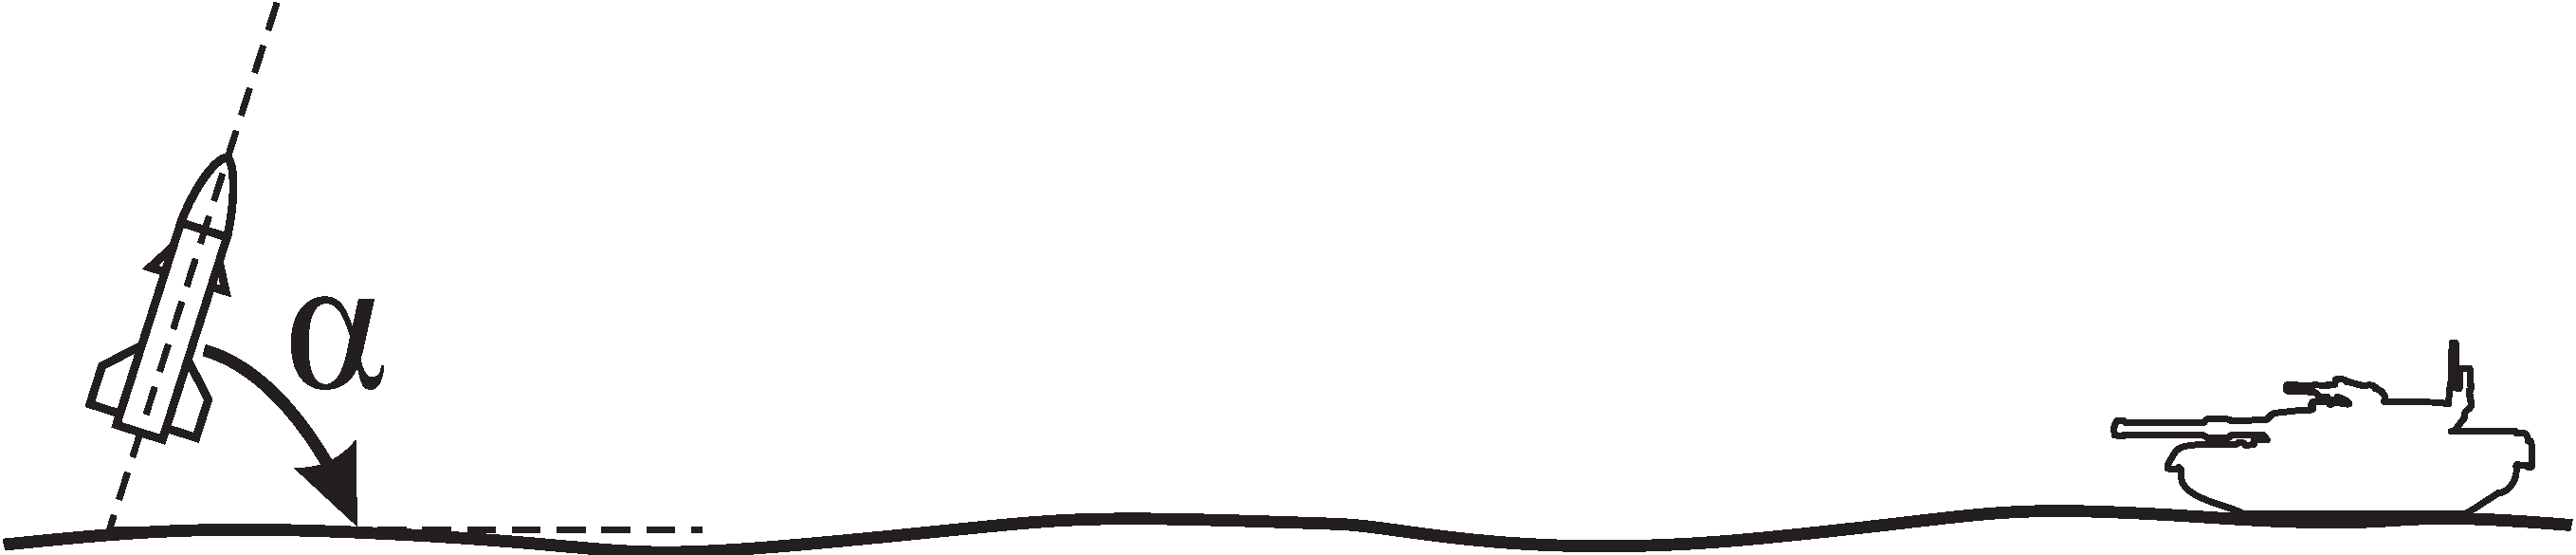
\includegraphics[width=0.475\textwidth]{rys05/alfa1}}}} 
%   \end{tabular}
%  a) trzy podejścia, b) podejście praktyczne}
%  \label{fig:alfabeta}
% \end{figure}
% \end{lstlisting}

% \begin{figure}[ht]
% 	\centering
% 		
\includegraphics[width=0.3\linewidth]{rys05/kanji-giri}
% 	\caption{Dwa znaki kanji -- giri}
% 	\label{fig:kanji-giri}
% \end{figure}

% \begin{figure}[htb]
%   \centering
% 	\begin{tabular}{@{}ll@{}}
% 	a) & b) \\
%   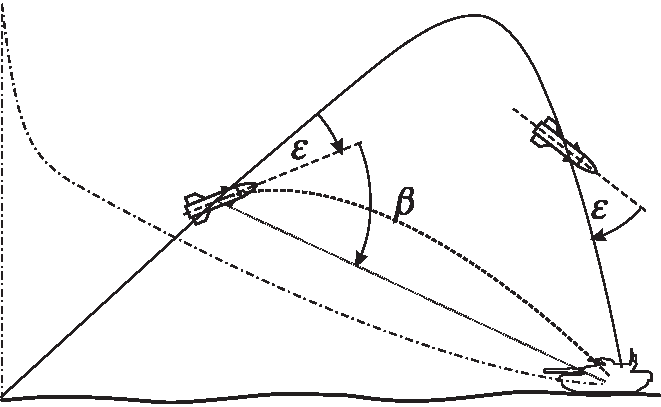
\includegraphics[width=0.475\textwidth]{rys05/beta1} & 
% 	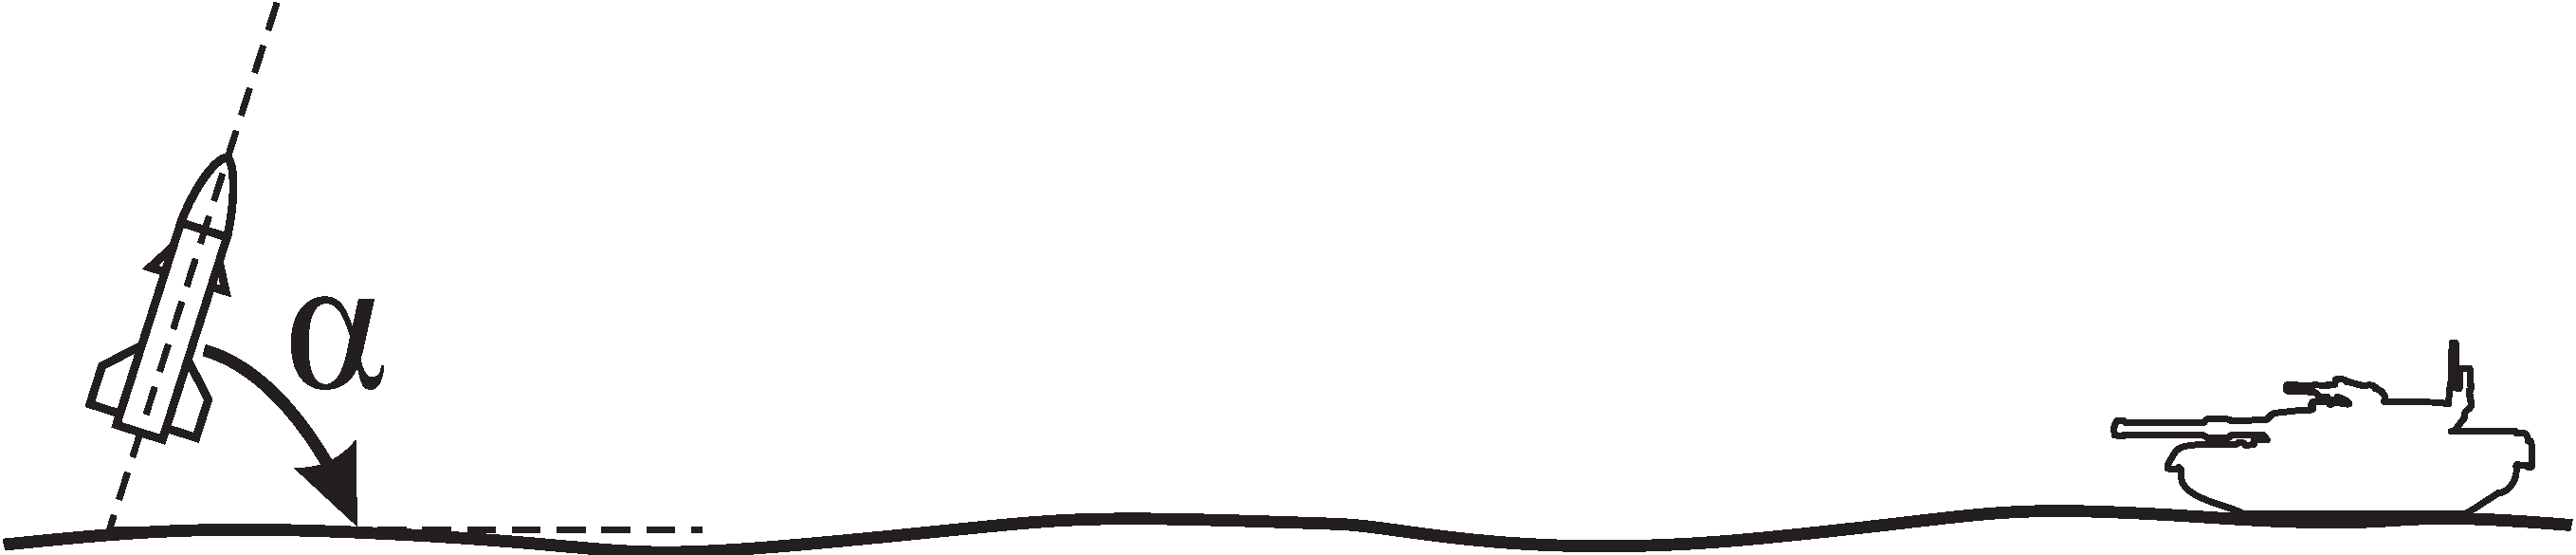
\includegraphics[width=0.475\textwidth]{rys05/alfa1}
% 	% jeśli obraki są różnej wysokości, można je wyrównać do góry stosując vtop jak niżej
% 	% \vtop{\vskip-2ex\hbox{{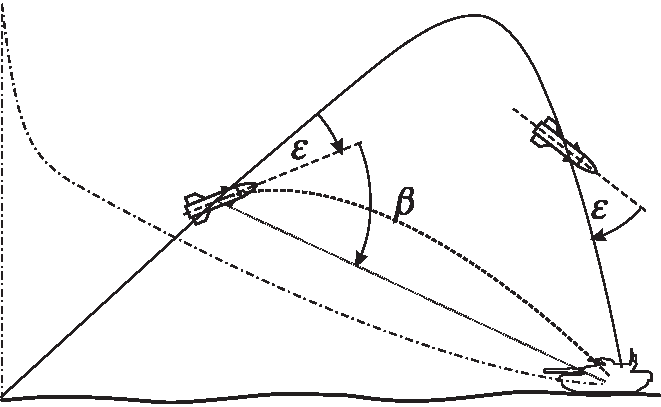
\includegraphics[width=0.475\textwidth]{rys05/beta1}}}} &
% 	% \vtop{\vskip-2ex\hbox{{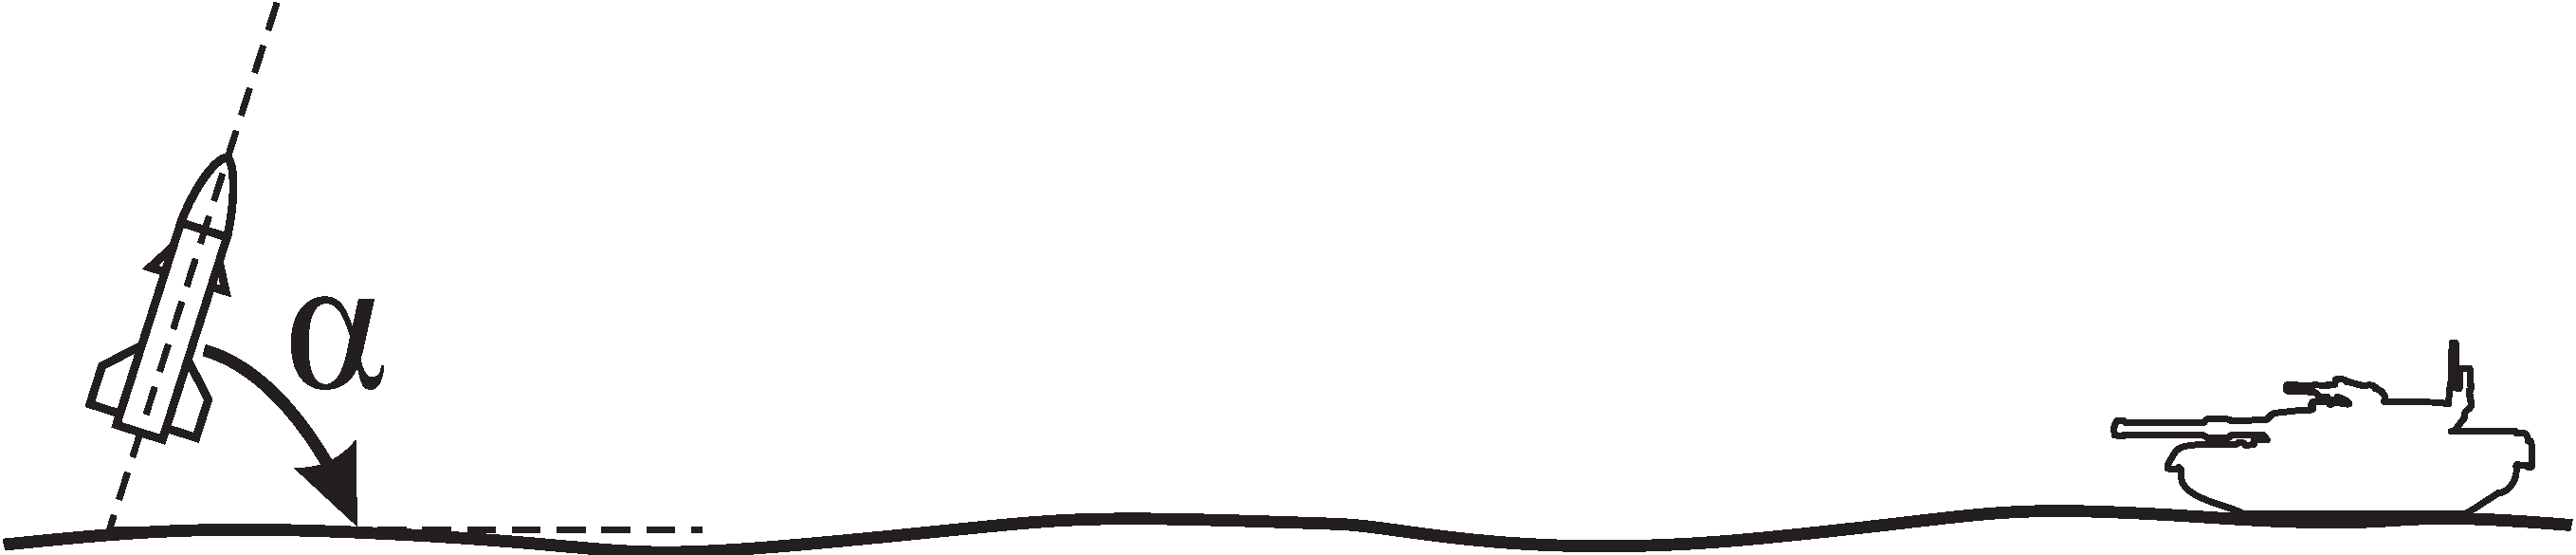
\includegraphics[width=0.475\textwidth]{rys05/alfa1}}}}  \caption{Wyznaczanie trajektorii lotu rakiety: 
% 	\end{tabular}
%   \caption{Wyznaczanie trajektorii lotu rakiety: a) trzy podejścia, b) podejście praktyczne}
%   \label{fig:alfabeta}
% \end{figure}

% Grafiki wektorowe powinny być dostarczone w plikach pdf. Rozmiar strony w~pliku pdf powinien być równy lub minimalnie większy od rozmiaru znajdującej się na nim grafiki (proszę spojrzeć na przykłady grafik wykorzystanych w niniejszym szablonie). Chodzi o to, aby na rysunku nie pojawiała się niepotrzebna biała przestrzeń (rozmiar płótna ma odpowiadać rozmiarowi grafiki bez żadnych marginesów, elementy grafiki powinny być ciasno ułożone). Grafiki rastrowe (głównie zrzuty z ekranu bądź zdjęcia) powinny być dostarczane w plikach o formacie \texttt{png} z~kompresją bezstratną. Zastosowanie kompresji stratnej, jak \texttt{jpg}, wprowadza niepotrzebne artefakty. Podobnie jak w przypadku grafik wektorowych, grafiki rastrowe nie powinny mieć białych marginesów.

% Niezłym sposobem generowanie ładnej grafiki wektorowej, w szczególności diagramów, jest posłużenie się, kolejno, następującymi darmowymi narzędziami:
% \begin{itemize}
% \item w \texttt{diagrams.net} (dawniej \texttt{draw.io}): narysowanie diagramu i wyeksportowanie do pdf (bezpośrednio lub pośrednio, poprzez zapisanie pliku w formacie \texttt{svg}, a potem jego wyświetlenie w~przeglądarce internetowej i wydrukowanie do \texttt{pdf}),
% \item w \texttt{inkscape}: zaimportowanie \texttt{pdf}, rozdzielenie grupy, wykasowanie niepotrzebnych elementów (tła), zaznaczenie wszystkiego, przycięcie strony do zaznaczonych (Ctr-Shift-R), zapisanie jako \texttt{pdf}. 
% \end{itemize}

% Na rysunku~\ref{fig:diagramy} pokazano przykład dobrze i źle (od strony technicznej) narysowanego diagramu. Celowo pokazano ramki, by było widać marginesy. Normalnie ramek tych nie należy stosować.
% \begin{figure}[htb]
%   \centering
% 	\begin{tabular}{@{}ll@{}}
% 	a) & b) \\
%   \vtop{\vskip-2ex\hbox{\fbox{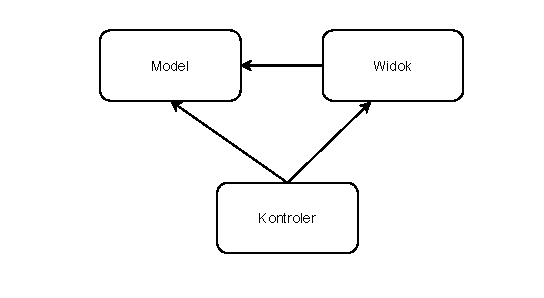
\includegraphics[width=0.4\linewidth]{rys05/diagram1}}}} & 
% 	\vtop{\vskip-2ex\hbox{\fbox{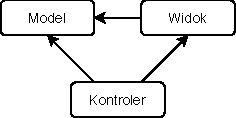
\includegraphics[width=0.4\linewidth]{rys05/diagram2}}}}
% 	% jeśli obraki są różnej wysokości, można je wyrównać do góry stosując vtop jak niżej
% 	% \vtop{\vskip-2ex\hbox{{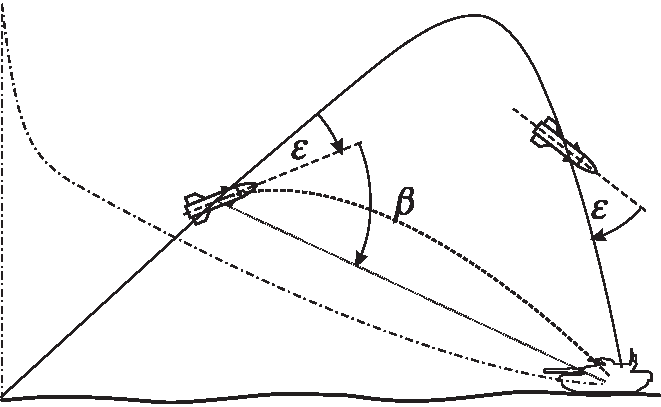
\includegraphics[width=0.475\textwidth]{rys05/beta1}}}} &
% 	% \vtop{\vskip-2ex\hbox{{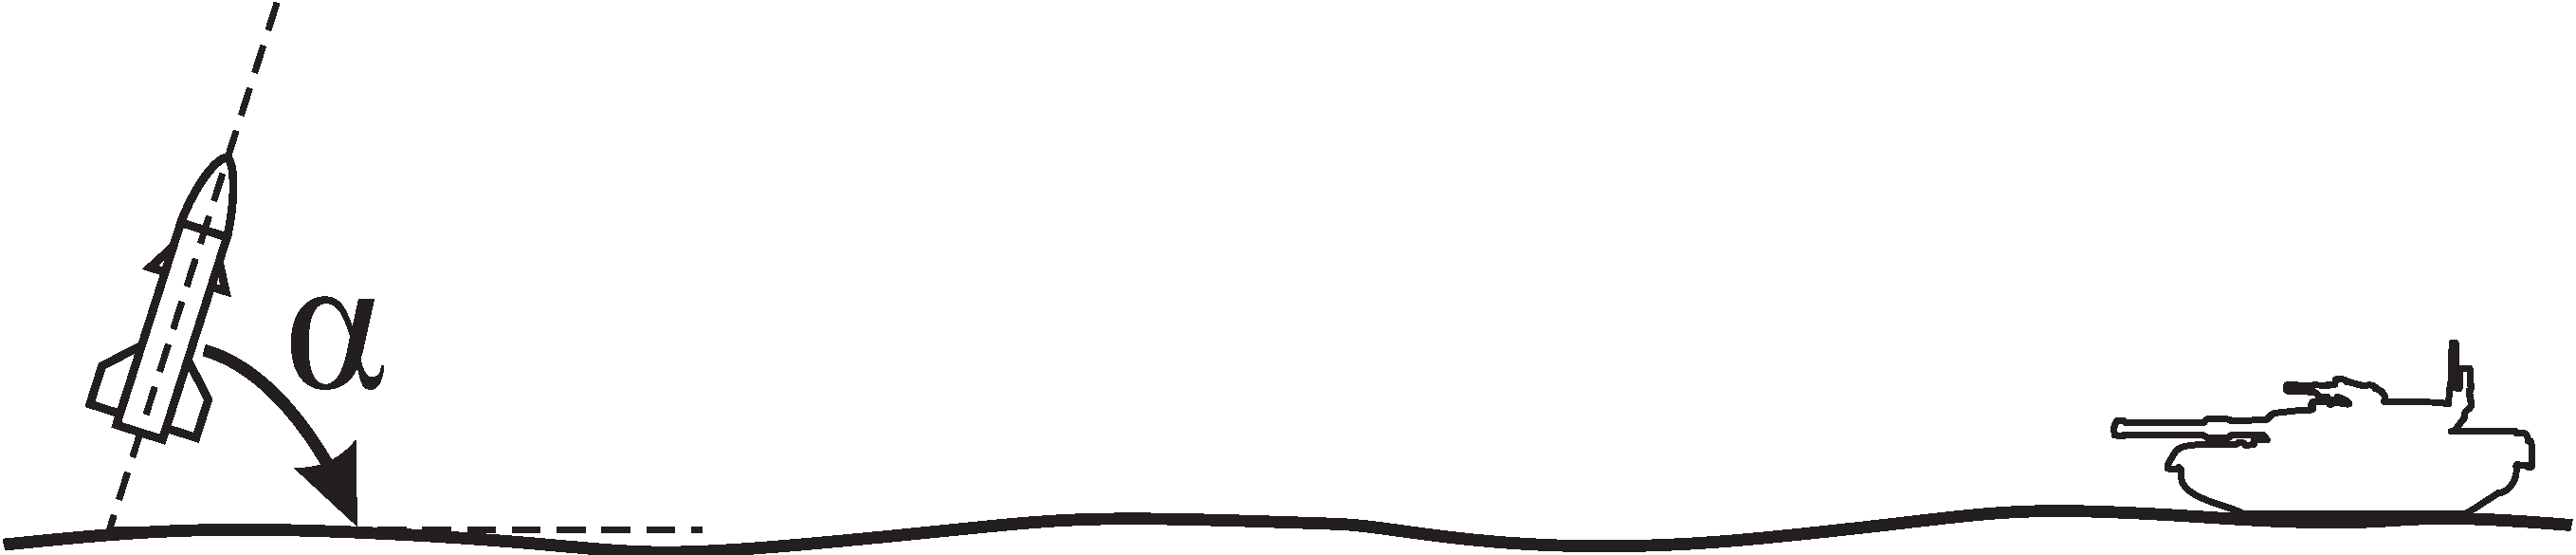
\includegraphics[width=0.475\textwidth]{rys05/alfa1}}}}  \caption{Wyznaczanie trajektorii lotu rakiety: 
% 	\end{tabular}
%   \caption{Przykład diagramu: a) złego, b) w miarę dobrego}
%   \label{fig:diagramy}
% \end{figure}

% Elementy na rysunkach nie powinny być wypełnione 100\% czernią ponieważ na wydrukach tworzą się plamy przebijające się przez kartkę. Zamiast tego wypełnienie elementów powinno być ustawione na ok.\ 90\% czerni.

% Czcionka na rysunkach nie może być większa od czcionki wiodącej tekstu (jedyny wyjątek to np.\ jakieś nagłówki).
% Należy stosować czcionkę kroju Arial, Helvetica bądź tego samego kroju co czcionka dokumentu (\texttt{texgyre-termes}). 

% Jeśli na jednym rysunku pojawić się ma kilka grafik, to zamiast stosować \texttt{subfigure} lub inne otoczenia należy: dostarczyć tabelę z wstawionymi do niej rysunkami, opcjonalnie adnotować jej części (np.~a) i b)), odnieść się do tych części w podpisie (posługując się adnotacjami, jak to zrobiono na rysunkach~\ref{fig:alfabeta} i \ref{fig:diagramy}, lub opisem słownym, np.~,,z lewej strony pokazano ...'', ,,po prawej zamieszczono ...'').

% Jeśli na rysunku zamieszczono w tabeli kilka grafik, to ich pozycjonowaniem (wyjustowaniem od góry) można manipulować za pomocą komendy:
% \verb+\vtop{\vskip-2ex\hbox{\includegraphics[width=0.475\textwidth]{nazwa}}}+

% Na rysunkach nie wolno nadużywać kolorów oraz ozdobników (wiele narzędzi do tworzenia diagramów dostarcza grafikę z cieniowaniem, gradacją kolorów itp.\  co niekoniecznie przekłada się na czytelność rysunku).
% Jeśli rysunki są kolorowe, to kolory te powinny być rozróżnialne po konwersji do poziomów szarości (chodzi o to, aby na wydrukach wykonanych na drukarkach monochromatycznych można było dostrzec różnice).

% Podczas robienia zrzutów z ekranu należy zadbać o to, by taki zrzut był czytelny po wydrukowaniu. Czyli aby pojawiające się literki były wystarczająco duże, a przestrzenie bez treści -- relatywnie małe. Przystępując do robienia zrzutu trzeba odpowiednio wyskalować elementy na ekranie. Na przykład robiąc zrzut z przeglądarki FF najpierw należy wcisnąć CTR--0 (domyślne skalowanie), potem CTR--{}- (zmniejszenie skali o stopień). Potem dobrze jest zawęzić okno przeglądarki tak, by interesująca treść wypełniła je w całości. Jeśli na obserwowanej stronie jest zbyt dużo pustych obszarów, to należy je jakoś zawęzić (sterując wielkością okna przeglądarki lub aktywnymi elementami interfejsu użytkownika). Zrzut bowiem wcale nie musi być odzwierciedleniem 1:1 domyślnego układu obserwowanych elementów. Ważne jest, by na zrzucie pokazać interesujący, opisywany fragment i żeby ten fragment był czytelny. Nie trzeba też zawsze robić zrzutów w układzie 16:9 (lub innym panoramicznym). Czasem lepiej jest zrobić zrzuty okien niemal kwadratowych, bo lepiej się układają w wynikowym dokumencie. Poza tym można je przeskalować (powiększyć) by zajmowały całą szerokość strony, a wtedy czcionka na wydrukach będzie większa. Takie skalowanie dla zrzutów panoramicznych zwykle się nie udaje. Na rysunku~\ref{fig:zrzuty} pokazano przykłady dobrze i źle zrobionych zrzutów (w celu oszczędzenia miejsca zrzuty umieszczono obok siebie).
% 	
% \begin{figure}[htb]
%   \centering
% 	\begin{tabular}{@{}ll@{}}
% 	a) & b) \\
%   \vtop{\vskip-2ex\hbox{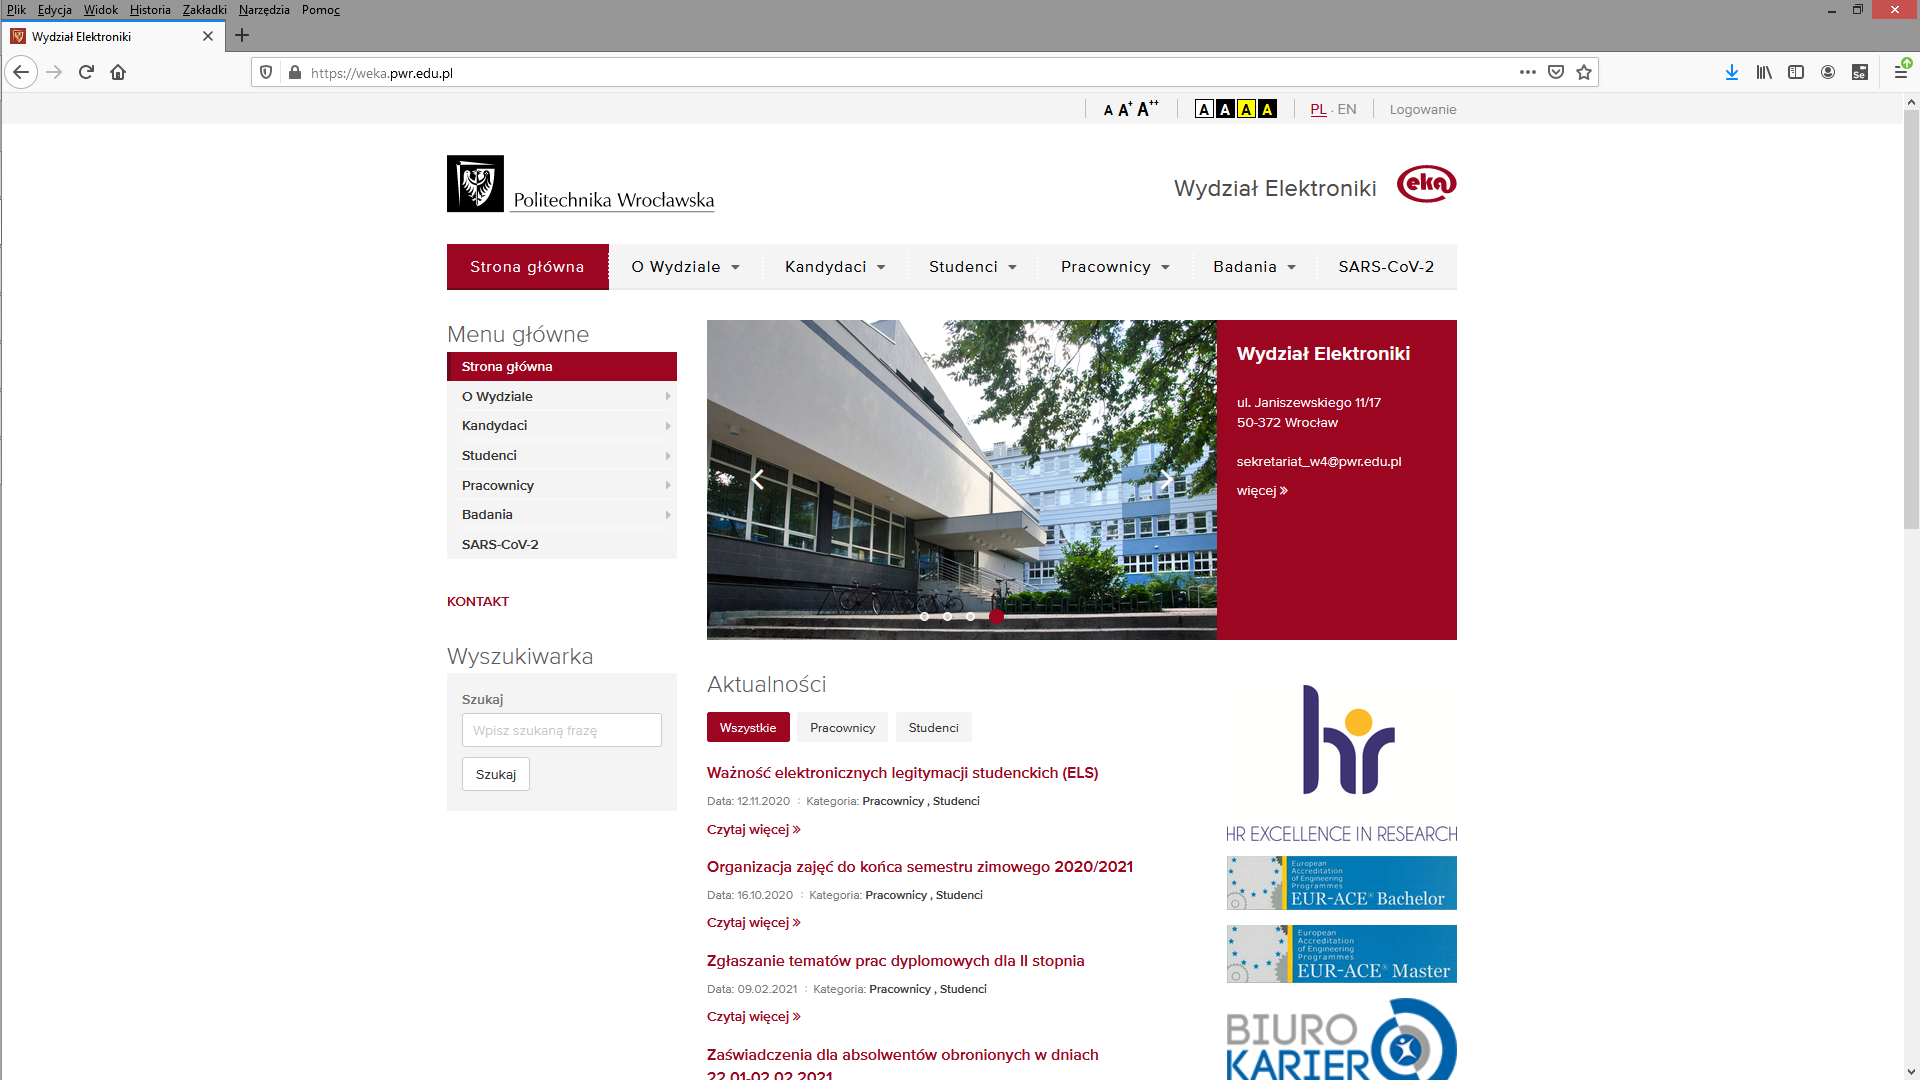
\includegraphics[width=0.475\textwidth]{rys05/zrzut1}}} & 
% 	\vtop{\vskip-2ex\hbox{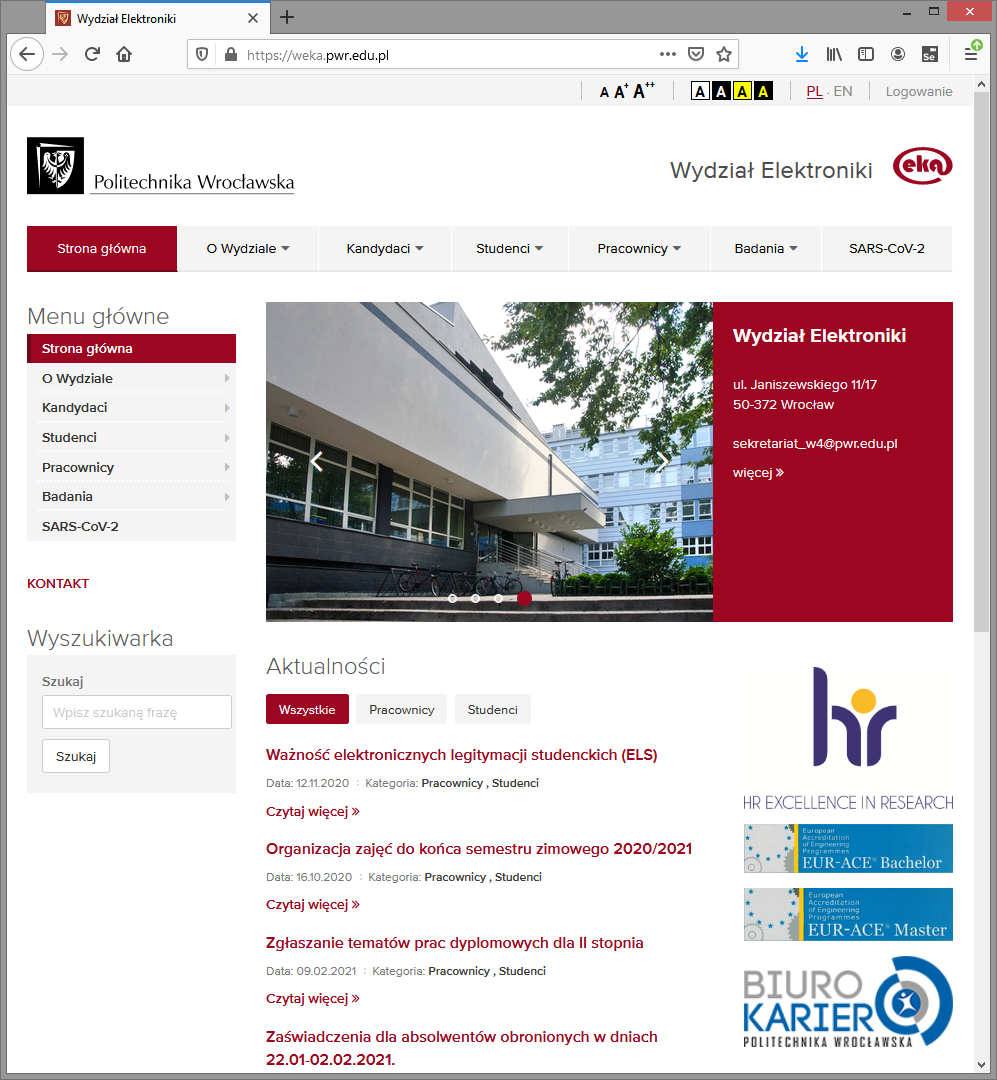
\includegraphics[width=0.475\textwidth]{rys05/zrzut2}}}
% 	% jeśli obraki są różnej wysokości, można je wyrównać do góry stosując vtop jak niżej
% 	% \vtop{\vskip-2ex\hbox{{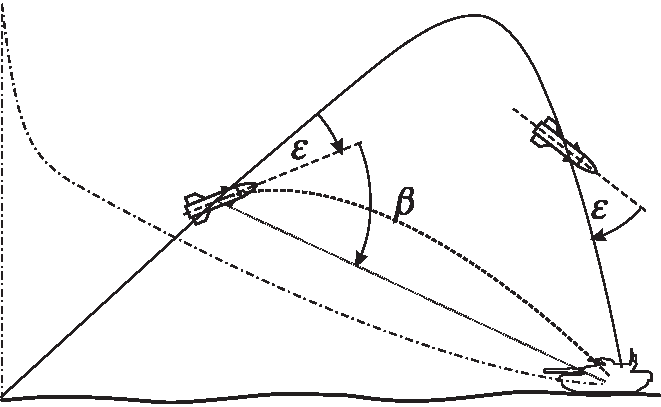
\includegraphics[width=0.475\textwidth]{rys05/beta1}}}} &
% 	% \vtop{\vskip-2ex\hbox{{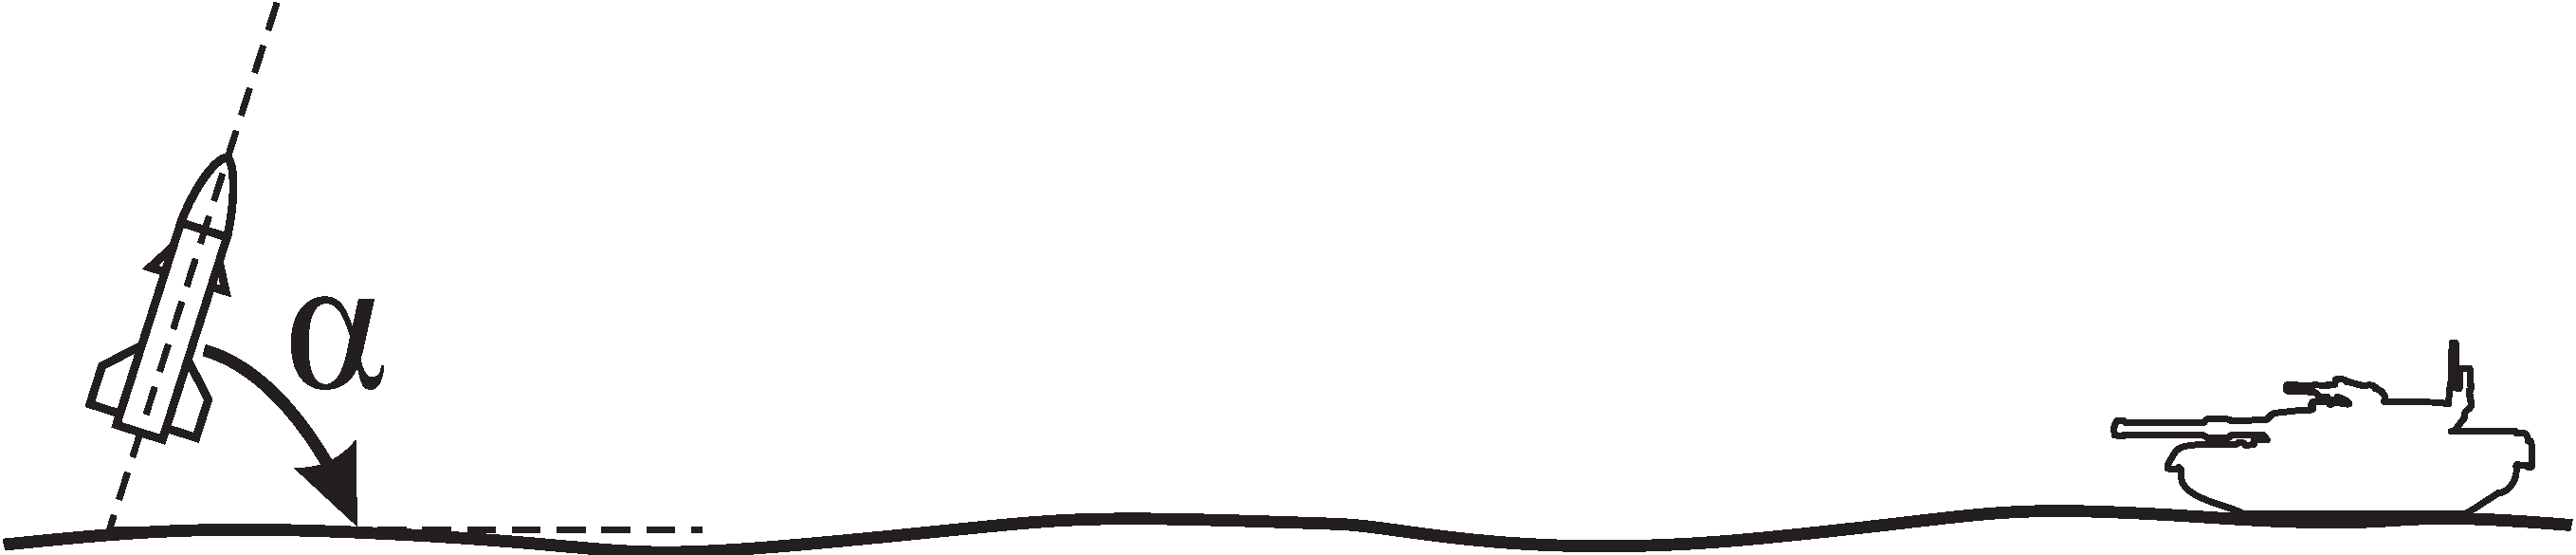
\includegraphics[width=0.475\textwidth]{rys05/alfa1}}}}  \caption{Wyznaczanie trajektorii lotu rakiety: 
% 	\end{tabular}
%   \caption{Przykłady zrzutów z ekranu: a) zły (nieczytelny, zrobiony przy zbyt szerokim oknie, z niepotrzebnymi marginesami, niepotrzebnym paskiem menu), b) w miarę dobry (w miarę czytelny, zrobiony przy zawężonym oknie, byłoby wskazane jeszcze usunięcie z niego beleczki z faviconem (jeśli nic nie wnosi) oraz przycięcie od dołu (jeśli treści tam pokazywane nie są istotne))}
%   \label{fig:zrzuty}
% \end{figure}

% 	
% Czasem problemem jest tworzenie zrzutów z ekranu, gdy występują na nim dane wrażliwe. Istnieją dwa sposoby na radzenie sobie z tym problemem.
% Pierwszy polega na zastąpieniu w~systemie danych danych rzeczywistych danymi testowymi -- wygenerowanymi tylko do celów prezentacji.
% Zrzut robi się wtedy na bazie danych testowych.
% Drugi polega na wykonaniu zrzutu z~ekranu, na którym pokazano dane rzeczywiste, i następnie zamianie tych danych już w pliku graficznym
% za pomocą odpowiedniego edytora (np.~\texttt{gimp}). Czyli oryginalny zrzut z ekranu należy otworzyć w edytorze, a potem
% nadpisać oryginalny tekst własnym tekstem. Konieczne jest wtedy dobranie odpowiednich czcionek aby nie było widać
% wprowadzonych zmian. 
% \begin{quotation}
% Uwaga: takie manipulowanie zrzutami jest usprawiedliwione jedynie w przypadku konieczności ochrony danych wrażliwych czy też lepszego pokazania wybranych elementów. Nie może to prowadzić generowania fałszywych rezultatów!!!
% \end{quotation}

% \section{Wstawianie kodu źródłowego}
% Kod źródłowy można wstawiać jako blok tekstu pisany czcionką maszynową. Używa się do tego otoczenie \verb?\lstlisting?. W atrybutach otoczenia można zdefiniować tekst podpisu wstawianego wraz z numerem nad blokiem, etykietę do tworzenia odwołań, sposób formatowania i~inne ustawienia. Zaleca się stosowanie w tym otoczeniu następujących parametrów:
% \begin{lstlisting}[basicstyle=\footnotesize\ttfamily]
% \begin{lstlisting}[label=list:req1,caption=Initial HTTP Request,
%                    basicstyle=\footnotesize\ttfamily]
% \end{lstlisting}
% Szczególnie przydatne podczas wstawiania większej ilości kodu źródłowego jest zastosowanie parametru \verb+basicstyle=\footnotesize\ttfamily+. Dzięki niemu zmniejsza się czcionka, a~przez to na stronie można zmieścić dłuższe linijki kodu. Użycie tak zdefiniowanego parametru nie jest jednak sztywnym zaleceniem. Wielkość czcionki można dobierać do potrzeb. 
% {\belowcaptionskip=-10pt
% \begin{lstlisting}[label=list:req1,caption=Initial HTTP Request,
%                    basicstyle=\footnotesize\ttfamily]
% GET /script/Articles/Latest.aspx HTTP/1.1
% Host: www.codeproject.com
% Connection: keep-alive
% Cache-Control: max-age=0
% Accept: text/html,application/xhtml+xml,application/xml
% User-Agent: Mozilla/5.0 ...
% Accept-Encoding: gzip,deflate,sdch
% Accept-Language: en-US...
% Accept-Charset: windows-1251,utf-8...
% \end{lstlisting}
% }
% Można też sformatować kod bez stosowania numerowanego podpisu (wtedy nie zamieszcza się \texttt{caption} na liście atrybutów).
% \begin{lstlisting}[basicstyle=\footnotesize\ttfamily]
% GET /script/Articles/Latest.aspx HTTP/1.1
% Host: www.codeproject.com
% Connection: keep-alive
% Cache-Control: max-age=0
% Accept: text/html,application/xhtml+xml,application/xml
% User-Agent: Mozilla/5.0 ...
% Accept-Encoding: gzip,deflate,sdch
% Accept-Language: en-US...
% Accept-Charset: windows-1251,utf-8...
% \end{lstlisting}

% Ponadto istnieje kilka sposobów wstawiania kodu źródłowego w bieżącej linijce tekstu:
% \begin{itemize} 
% \item korzystając z polecenia \verb?\texttt? ustawiającego czcionkę maszynową, jak w przykładzie \texttt{tutaj} (efekt zastosowania komendy \verb?\texttt{tutaj}?). Problemem jednak mogą okazać się znaki podkreślenia i inne znaki kontrolne.
% \item korzystają z otoczenia \verb?\verb? zapewniającego wypisanie kodu czcionką maszynową jak w~przykładzie \verb|tutaj| (efekt zastosowania komendy \verb?\verb|tutaj|?). Problemem jest to, że polecenie \verb?\verb? nie potrafi łamać dłuższego tekstu.
% \item korzystając z polecenia \verb?\lstin? umożliwiającego wypisanie kodu czcionką ustawianą w~opcjach jak w przykładzie
% \lstset{basicstyle=\ttfamily}\lstinline{tutaj} (efekt komendy \verb+\lstset{basicstyle=\ttfamily}\lstinline{tutaj}+) lub \lstinline[basicstyle=\ttfamily]=tutaj= (efekt komendy \verb+\lstinline[basicstyle=\ttfamily]=tutaj=+).
% \end{itemize}

% Poniżej zamieszczono przykłady kodów źródłowych z podświetleniem składni.

% \begin{lstlisting}[language=Java,style=JavaStyle,caption=Opis 1, label=lst:pierwszy]
% package pl.mrbarozoit.backend;

% import org.springframework.boot.SpringApplication;
% import org.springframework.boot.autoconfigure.SpringBootApplication;

% @SpringBootApplication
% public class BackendApplication {

%     public static void main(String[] args) {
%         SpringApplication.run(BackendApplication.class, args);
%     }

% }
% \end{lstlisting}

% Jeśli w kodzie źródłowym jest jakiś nieistotny fragment względem omawianego problemu, to można go wykropkować (patrz listing~\ref{lst:drugi}).

% {\belowcaptionskip=-9pt % To polecenie zmniejszy odległość podpisu od pokazywanego kodu (jego stosowanie jest zalecane)
% \begin{lstlisting}[language=JavaScript,style=JavaScriptStyle,caption=Opis 2, label=lst:drugi]
% // Karma configuration file, see link for more information
% // https://karma-runner.github.io/1.0/config/configuration-file.html

% module.exports = function (config) {
%   config.set({
%     basePath: '',
%     frameworks: ['jasmine', '@angular-devkit/build-angular'],
%     plugins: [
%       require('karma-jasmine'),
%       require('karma-chrome-launcher'),
%       require('karma-jasmine-html-reporter'),
%       require('karma-coverage-istanbul-reporter'),
%       require('@angular-devkit/build-angular/plugins/karma')
%     ],
%     ... // opuszczony kod
%     autoWatch: true,
%     browsers: ['Chrome'],
%     singleRun: false,
%     restartOnFileChange: true
%   });
% };
% \end{lstlisting}
% }

% Jeśli kod jest wąski, to można sformatować go w dwóch kolumnach jak na listingu~\ref{lst:kontrakt-board-move-in}.

% % Trzeba zacząć po linijce przerwy
% \begingroup 
% \listingcaption{Kontrakt na model wejściowy endpointu \texttt{/api/v1/chess/board/move}}
% \setlength\multicolsep{0pt plus 2pt}%
% \begin{lstlisting}[style=json-style, multicols=2, label=lst:kontrakt-board-move-in]
% {
%    "lastPosition": {
%       "fenDescription": "string"
%    },
%    "image": {
%       ...
%    },
%    "positions": {
%       "chessboardCorners": [
%          ...
%       ],
%       "tilesCornerPoints": [
%          ...
%       ]
%    },
%    "referenceColors": {
%       ...
%    },
% }
% \end{lstlisting}
% \vspace{6pt plus 2pt}
% \endgroup

% \section{Wykaz literatury oraz cytowania}
% \label{sec:literatura}
% Cytowania powinny być zamieszczane w tekście z użyciem komendy \verb+\cite{}+. Jej argumentem powinien być klucz cytowanej pozycji (lub lista kluczy  rozdzielonych przecinkiem bez spacji, jeśli takich pozycji w danym miejscu cytuje się więcej) jaki jest używany w bazie danych bibliograficznych (plik \texttt{dokumentacja.bib}). Po kompilacji \texttt{bibtex} i \texttt{pdflatex} w tekście pojawia się właściwy odsyłacz do pozycji w wykazie literatury (ujęty w kwadratowe nawiasy -- zgodnie z~tym, co definiuje styl \texttt{plabbrv.bst}), zaś w samym wykazie (rozdział Literatura) -- zacytowana pozycja. Przykładem cytowania jest: ,,dobrze to opisano w pracach~\cite{JS07,SQL2}'' (gdzie zastosowano komendę \verb?\cite{JS07,SQL2}?).

% Co do zawartości rekordów bibliograficznych - style bibtexowe potrafią ,,skracać'' imiona (czyli wstawiać, jeśli taka wola, inicjały zamiast pełnych imion). Niemniej dobrze jest od razu przyjąć jakąś konwencję. Proponuje się, aby w rekordach od razu wstawiane były inicjały zamiast pełnych imion.

% Niekiedy tytuły prac zawierają wyrazy z dużymi i małymi literami. Takie tytuły należy brać w podwójne nawiasy klamrowe, aby \texttt{bibtex} nie zamienił ich na postać, w której poza pierwszą literą pozostałe są małe.

% Jeśli jakiś cytowany zasób pochodzi z Internetu, to jego rekord w pliku \texttt{bib} powinien wyglądać jak niżej.
% \begin{lstlisting}[basicstyle=\footnotesize\ttfamily]
% @INPROCEEDINGS{SQL2, 
%   title={{A MySQL-based data archiver: preliminary results}}, 
%   author={Bickley, M. and Slominski, Ch.},
%   booktitle = {{Proceedings of ICALEPCS07}},
% 	month = oct,
% 	day = {15--19},
% 	year={2007}, 
%   note={\url{http://www.osti.gov/scitech/servlets/purl/922267} 
% 	[dostęp dnia 20 czerwca 2015]}
% }
% \end{lstlisting}
% A to inny przykład rekordu danych bibliograficznych:
% \begin{lstlisting}[basicstyle=\footnotesize\ttfamily]
% @TechReport{JS07,
% 	author = {Jędrzejczyk, J. and Śródka, B.},
% 	title  ={Segmentacja obrazów metodą drzew decyzyjnych},
% 	year = {2007},
% 	institution = {Politechnika Wrocławska, Wydział Elektroniki}
% }
% \end{lstlisting}

% \section{Indeks rzeczowy}
% \label{sec:indeks}
% Generowanie indeksu \index{generowanie!-- indeksu} po trosze wygląda jak generowanie wykazu literatury \index{generowanie!-- wykazu literatury}-- wymaga kilku kroków. Podczas pierwszej kompilacji \texttt{pdflatex} generowany jest plik z rozszerzeniem \texttt{*.idx} (zawierający ,,surowy indeks''). Następnie, bazując na tym pliku, generowany jest plik z rozszerzeniem \texttt{*.ind} zawierający sformatowane dane. Ten krok wymaga uruchomienia odpowiedniego narzędzia oraz zastosowania plik z definicją stylu \texttt{Dyplom.ist}. W kroku ostatnim dokonuje się kolejnej kompilacji \texttt{pdflatex} (dzięki niej w wynikowym dokumencie pojawi się Indeks rzeczowy). Domyślnie Indeks rzeczowy zostanie sformatowany w~układzie dwukolumnowym.

% Oczywiście aby to wszystko zadziałało w kodzie szablonu należy umieścić odpowiednie komendy definiujące elementy indeksu rzeczowego (\verb?\index?) oraz wstawiające sformatowany Indeks rzeczowy do dokumentu wynikowego (\verb?\printindex?). Więcej informacji o tworzeniu indeksu rzeczowego można znaleźć na stronie \url{https://en.wikibooks.org/wiki/LaTeX/Indexing}. Poniżej przedstawiono przykłady komend użytych w szablonie do zdefiniowania elementów indeksu rzeczowego:
% \begin{itemize}
% \item \verb?\index{linia komend}? -- pozycji główna.
% \item \verb?\index{generowanie!-- indeksu}? -- podpozycja.
% \end{itemize}

% Generowanie pliku \texttt{*.ind} można inicjować na kilka sposobów:
% \begin{itemize}
% \item poprzez wydanie odpowiedniego polecenia bezpośrednio w linii komend \index{linia komend}
% \begin{lstlisting}[basicstyle=\footnotesize\ttfamily]
% makeindex Dyplom.idx -t Dyplom.ilg -o Dyplom.ind -s Dyplom.ist
% \end{lstlisting}
% \item poprzez odpalenie odpowiedniego narzędzia środowiska. Na przykład w \texttt{TeXnicCenter} definiuje się tzw. \texttt{output profiles}: 
% \begin{lstlisting}[basicstyle=\footnotesize\ttfamily]
% makeindex "%tm.idx" -t "%tm.ilg" -o "%tm.ind" -s "%tm.ist"
% \end{lstlisting}
% a samo generowanie pliku \texttt{*.ind} zapewni wybranie pozycji menu \texttt{Build/Makeindex}.
% \item korzystając z odpowiednio sparametryzowanych pakietów i komend wewnątrz kompilowanego dokumentu (czyli od razu przy okazji jego kompilacji).
% \begin{lstlisting}[basicstyle=\footnotesize\ttfamily]
% \DisemulatePackage{imakeidx}
% \usepackage[noautomatic]{imakeidx} 
% % jeśli chcemy, by indeks by generowany automatycznie programem makeindex:
% %\usepackage[makeindex]{imakeidx} 
% % a tak ponoć można przekazać opcje do programu generującego indeks:
% %\makeindex[options=-s podrecznik -L polish -M lang/polish/utf8] 
% %\makeindex[options=-s podrecznik]
% \makeindex
% \end{lstlisting}

% Niestety, \texttt{makeindex} jest narzędziem, które umieszcza część pozycji w grupie \texttt{Symbols}, a~nie w grupach związanych z literkami alfabetu. W związku z czym indeksowany element zaczynający się od polskiej literki trafia do grupy \texttt{Symbols}, jak np.~\verb?\index{Światło}?\index{Światło}. Jeśli chce się zamieszczać w indeksie symbole matematyczne, to dobrze jest to robić jak w następującym przykładzie: \verb?\index{$asterisk@$\ast$}? \index{$asterisk@$\ast$} czy też \verb?\index{c@$\mathcal{C}$}?\index{c@$\mathcal{C}$}, tj.~dostarczając przy okazji klucz do sortowania.
% Lepiej w tym względzie radzą sobie inne narzędzia, jak \texttt{texindy} lub \texttt{xindy} dostępne pod linuxem. Korzystając z nich uzyskuje się grupy polskich literek w indeksie rzeczowym (hasła zaczynające się od polskich literek już nie trafiają do grupy Symbols). Przykład polecenia wydanego z linii komend, w którym wykorzystano \texttt{texindy} zamieszczono poniżej (zakładamy kodowanie plików w UTF8, można dla niniejszego szablonu zmienić na cp1250):
% \begin{lstlisting}[basicstyle=\footnotesize\ttfamily]
% texindy -L polish -M lang/polish/utf8 Dyplom.idx
% \end{lstlisting}

% To polecenie wygeneruje \texttt{Dyplom.ind} o zawartości:
% \begin{lstlisting}[basicstyle=\footnotesize\ttfamily]
% \begin{theindex}
%   \providecommand*\lettergroupDefault[1]{}
%   \providecommand*\lettergroup[1]{%
%       \par\textbf{#1}\par
%       \nopagebreak
%   }

%   \lettergroup{G}
%   \item generowanie
%     \subitem -- indeksu, 27
%     \subitem -- wykazu literatury, 27

%   \indexspace

%   \lettergroup{L}
%   \item linia komend, 27

%   \indexspace

%   \lettergroup{Ś}
%   \item \'Swiat\IeC {\l }o, 28

% \end{theindex}
% \end{lstlisting}


% \end{itemize}


% Aby mieć większą kontrolę automatyczne generowanie indeksu zostało w niniejszym szablonie wyłączone (indeks trzeba wygenerować samemu, wydając polecenie \texttt{makeindex} lub zalecane \texttt{texindy}).

% \section{Inne uwagi}
% Dobrym sposobem na kontrolę błędów występujących podczas kompilacji jest wstawianie linijki \verb?\end{document}? w wybranym miejscu dokumentu. Jest to szczególnie przydatne w przypadkach, gdy błędy te są trudne do zidentyfikowania (gdy wygenerowane przez kompilator numery linii z błędami nie są tymi, w których błędy występują). Wystarczy wtedy przestawić wspomnianą linijkę do kolejnych miejsc, aż znajduję to miejsce, gdzie występuje problem.

% Aby osiągnąć apostrofy maszynowe (złożone z samych kresek) należy użyć polecenia \verb?"{}jak tutaj{}"? (podwójny apostrof stojący bezpośrednio przed niektórymi literkami zamienia je na literki z akcentami, aby temu zapobiec dostawiono nawiasy klamrowe). W efekcie otrzymamy "{}jak tutaj{}". Jeśli natomiast apostrofy mają być drukarskie (złożone z kropek i kresek), to należy użyć polecenia \verb?,,jak tutaj''? (dwa pojedyncze przecinki i dwa pojedyncze apostrofy). W efekcie otrzymamy ,,jak tutaj''. Można też użyć znaków apostrofów odpowiednio zakodowanych „jak tutaj”, tylko że czasem trudno pisze się takie apostrofy w środowiskach kompilacji projektów latexowych.


% Oto sposoby ustawienia odstępów między liniami:
% \begin{itemize}
% \item używając komendy \verb+\linespread{...}+ (akceptowalne), przy czym atrybutem tej metody jest współczynnik zależny od wielkości
% czcionki.  Dla czcionki wiodącej 12pt odstęp półtora linii osiągnie się komendą \verb+\linespread{1.241}+. Dla innych czcionek wiodących wartości tego parametru są jak w poniższym zestawieniu.
% \begin{lstlisting}[basicstyle=\footnotesize\ttfamily]
% 10pt 1.25 dla \onehalfspacing 
%      1.667 for \doublespacing, 
% 		 ponieważ ,,basic ratio'' = 1.2 
% 		(\normalfont posiada \baselineskip rozmiaru 12pt)
% 11pt 1.213 dla \onehalfspacing oraz 1.618 dla \doublespacing, 
%      ponieważ ,,basic ratio'' = 1.236 
% 		(\normalfont posiada \baselineskip rozmiaru 13.6pt)
% 12pt 1.241 dla \onehalfspacing oraz 1.655 dla \doublespacing, 
%      ponieważsince ''basic ratio'' is 1.208 
% 		(\normalfont has a \baselineskip of 14.5pt)
% \end{lstlisting}
% Kłopot w tym, że raz ustawiony odstęp będzie obowiązywał do wszystkich czcionek (brak jest mechanizmu zmiany współczynnika w zależności od wielkości czcionki akapitu).

% \item używając pakietu \texttt{setspace} (niezalecane). Ponieważ klasa \texttt{memoir} emuluje pakiet \texttt{setspace}, w preambule dokumentu należałoby umieścić:
% \begin{lstlisting}[basicstyle=\footnotesize\ttfamily]
% \DisemulatePackage{setspace}
% \usepackage{setspace}
% \end{lstlisting}
% a potem można już sterować odstęp komendami:
% \begin{lstlisting}[basicstyle=\footnotesize\ttfamily]
% \singlespacing
% \onehalfspacing
% \doubelspacing
% \end{lstlisting}
% Ten sposób pozwala na korzystanie z mechanizmu automatycznej zmiany odległości linii w~zależności od wielkości czcionki danego akapitu.
% \item korzystając bezpośrednio z komend dostarczonych w klasie \texttt{memoir} (zalecane):
% \begin{lstlisting}[basicstyle=\footnotesize\ttfamily]
% \SingleSpacing
% \OnehalfSpacing
% \DoubleSpacing
% \end{lstlisting}
% Ten sposób również pozwala na korzystanie z mechanizmu automatycznej zmiany odległości linii w zależności od wielkości czcionki danego akapitu.
% \end{itemize}

% Na koniec jeszcze uwaga o rozmiarze pliku wynikowego. Otóż \texttt{pdflatex} generuje pliki \texttt{pdf}, które zazwyczaj mogłyby być nieco lepiej
% skompresowane. Do lepszego skompresowania tych plików można użyć programu \texttt{ghostscript}. Wystarczy w tym celu wydać komendę (pod windowsami):
% \begin{lstlisting}[basicstyle=\footnotesize\ttfamily]
% gswin64 -sDEVICE=pdfwrite -dCompatibilityLevel=1.4 -dNOPAUSE -dQUIET \
% -dSAFER -dBATCH -sOutputFile=Dyplom-compressed.pdf Dyplom.pdf
% \end{lstlisting}
% W poleceniu tym można również wstawić opcję \texttt{-dPDFSETTINGS=/prepress} (zapewniającą uzyskanie wysokiej jakości, zachowanie kolorów, uzyskanie obrazków w rozdzielczości 300 dpi). Ze względów licencyjnych ghostscript używa domyślnie algorytmów z kompresją stratną. Przy kompresji może więc dojść do utraty jakości bitmap.
